\documentclass[11pt]{article}
\usepackage[utf8]{inputenc}
\usepackage{amsmath,amsthm,amssymb}
\usepackage[usenames,dvipsnames]{xcolor}
\usepackage[colorlinks=true,citecolor=ForestGreen,linkcolor=ForestGreen,urlcolor=NavyBlue]{hyperref}
\usepackage{pgf,tikz,pgfplots}
\usetikzlibrary{matrix}
\usetikzlibrary{calc,patterns,intersections,pgfplots.fillbetween}
\usepackage[suppress]{color-edits}

\begin{document}

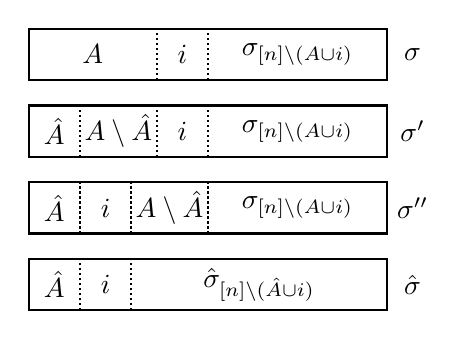
\begin{tikzpicture}[scale = 0.65,thick]
    % last rectangle
    \draw (0,0) rectangle (7,1);
    \node at (0.5,0.5) {$\hat A$};
    \node at (1.5,0.5) {$i$};
    \node at (4.5,0.5) {$\hat{\sigma}_{[n] \setminus (\hat A\cup i)}$};
    \node at (7.5,0.5) {$\hat \sigma$};
    \foreach \x in {1,2}
        \draw[densely dotted] (\x,0) -- (\x,1);
    
    % Third rectangle
    \draw (0,1.5) rectangle (7,2.5);
    \node at (0.5,2) {$\hat A$};
    \node at (1.5,2) {$i$};
    \node at (2.75,2) {${A} \setminus \hat{A} $};
    \node at (5.25,2) {$\sigma_{[n] \setminus (A\cup i)}$};
    \node at (7.5,2) {$\sigma''$};
    \foreach \x in {1,2,3.5}
        \draw[densely dotted] (\x,1.5) -- (\x,2.5);
    
    % Second rectangle
    \draw (0,3) rectangle (7,4);
    \node at (0.5,3.5) {$\hat A$};
    \node at (1.75,3.5) {${A} \setminus \hat{A} $};
    \node at (3,3.5) {$i$};
    \node at (5.25,3.5) {$\sigma_{[n] \setminus (A\cup i)}$};
    \node at (7.5,3.5) {$\sigma'$};
    \foreach \x in {1,2.5,3.5}
        \draw[densely dotted] (\x,3) -- (\x,4);
    
    % First rectangle
    \draw (0,4.5) rectangle (7,5.5);
    \node at (1.25,5) {$A$};
    \node at (3,5) {$i$};
    \node at (5.25,5) {$\sigma_{[n] \setminus (A\cup i)}$};
    \node at (7.5,5) {$\sigma$};
    \foreach \x in {2.5,3.5}
        \draw[densely dotted] (\x,4.5) -- (\x,5.5);
\end{tikzpicture}

\end{document}